\begin{FPfigure}

\begin{center}
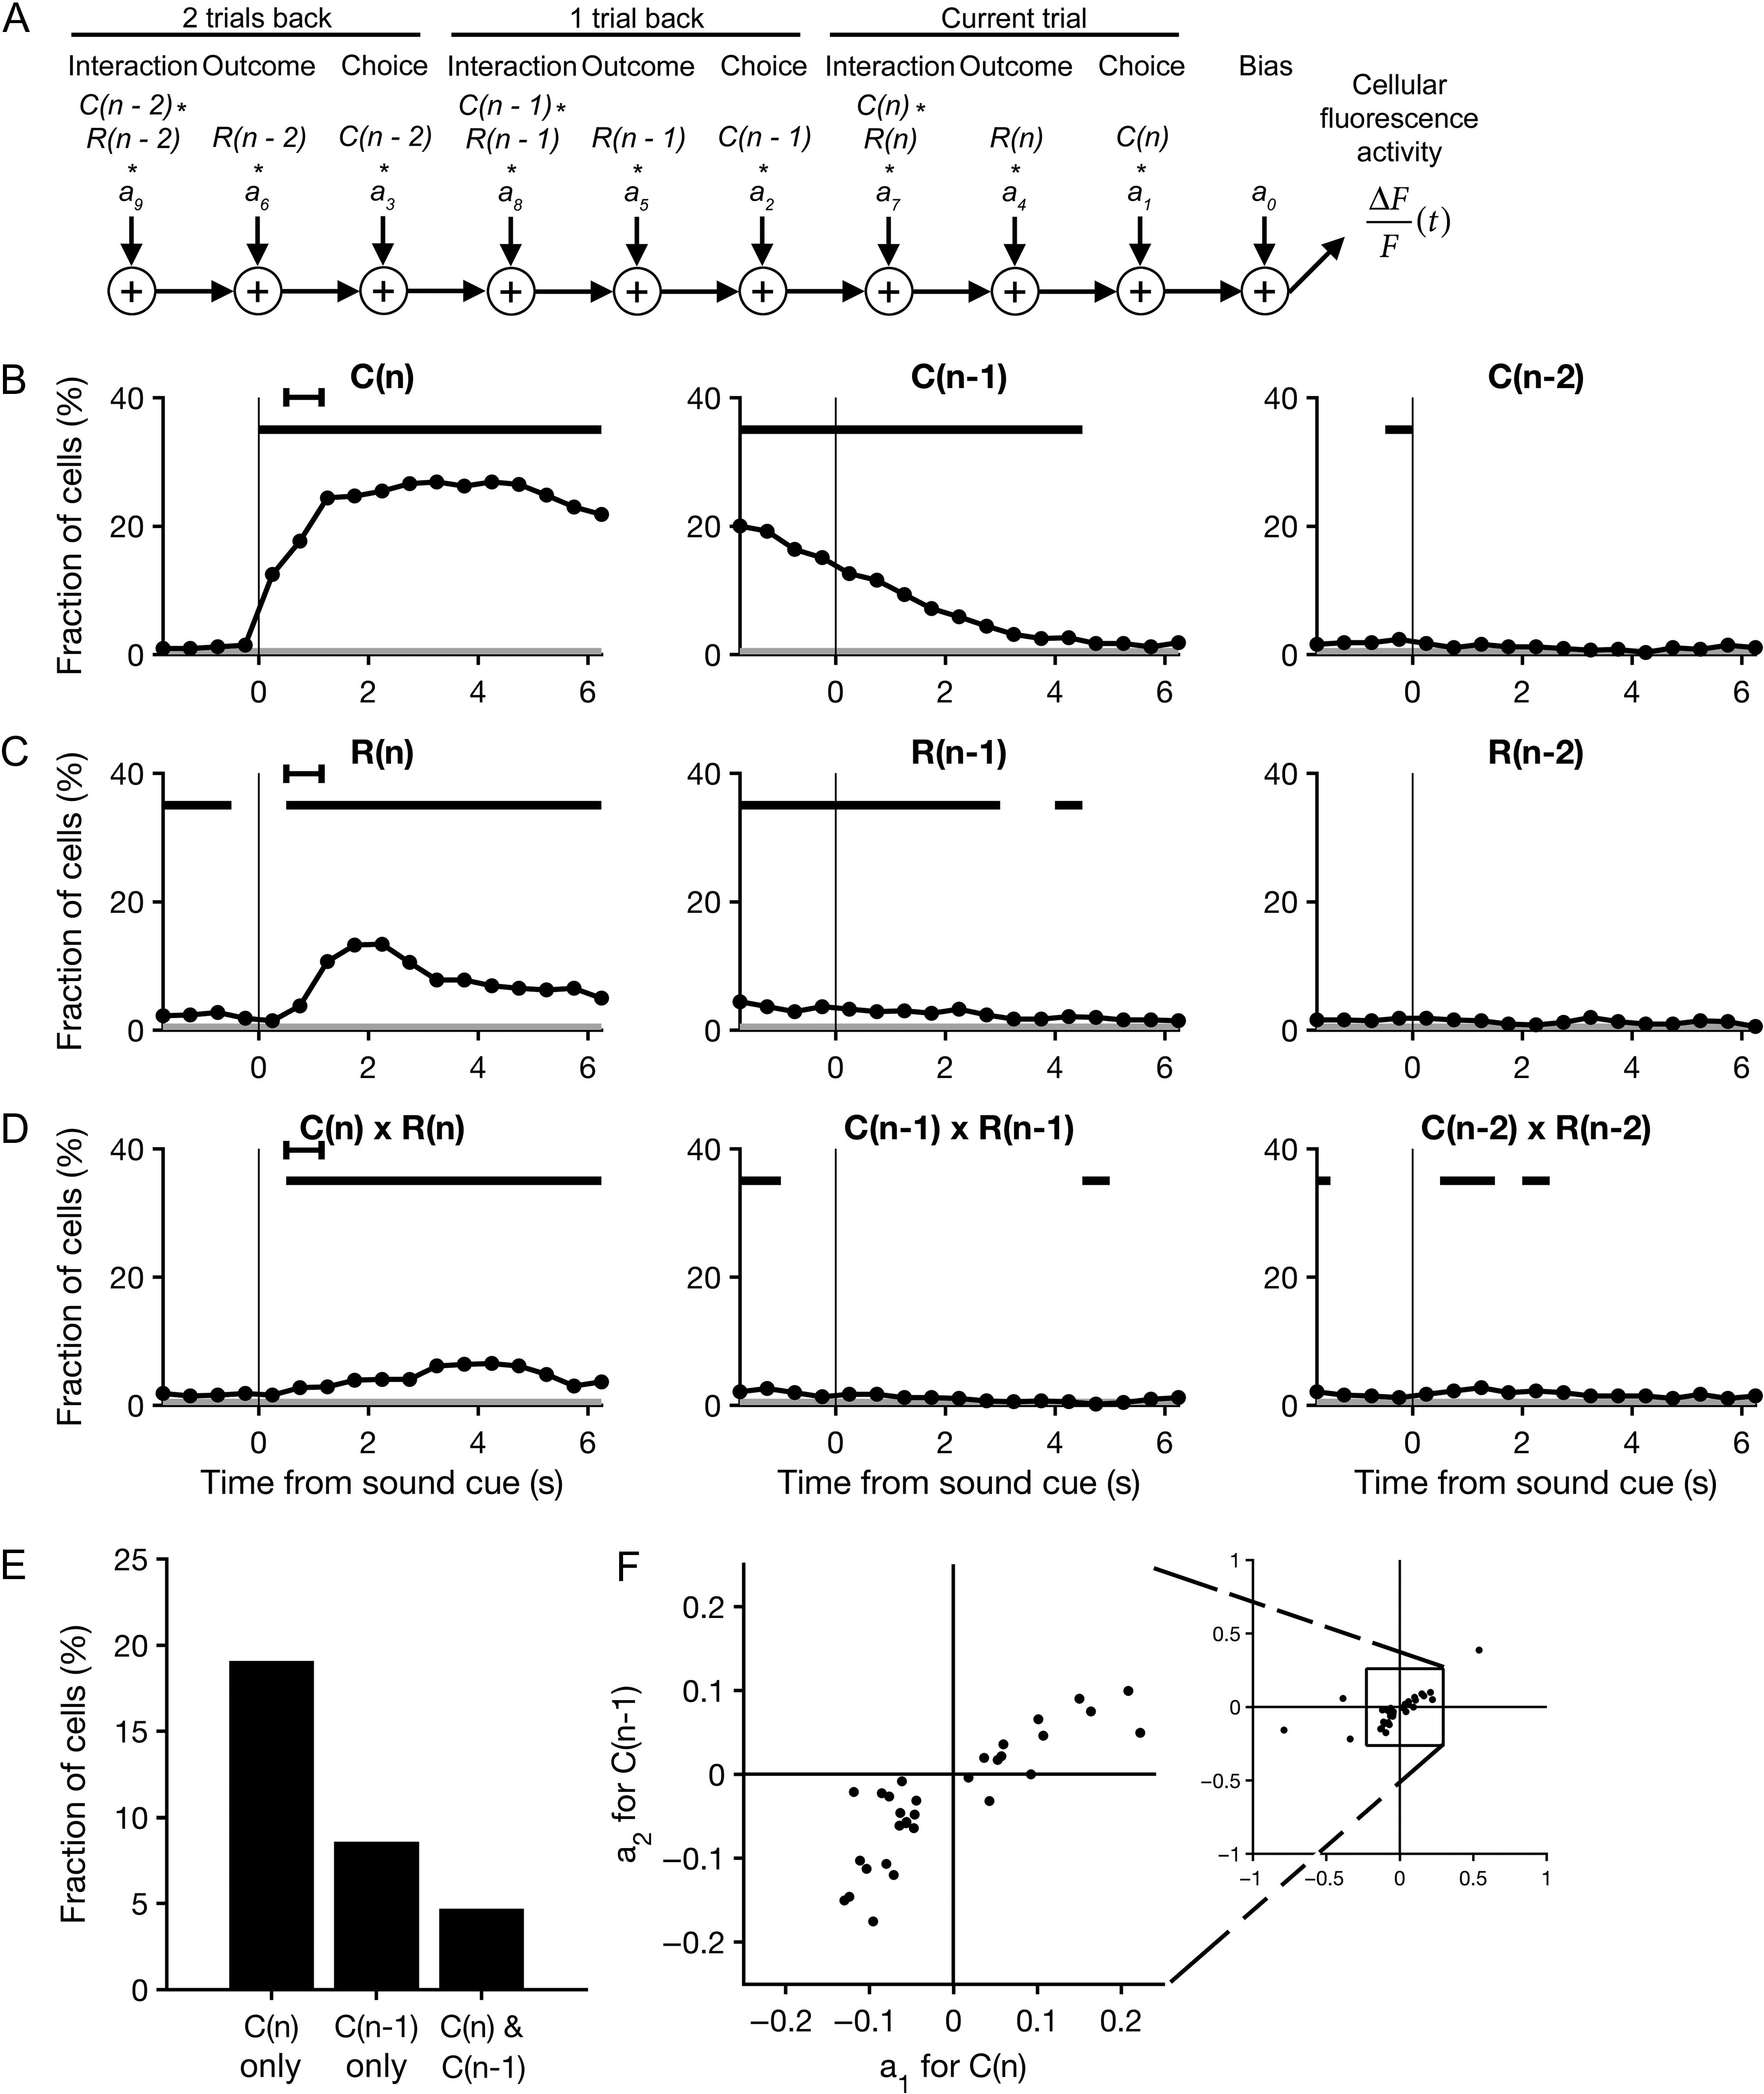
\includegraphics[width=\textwidth]{Figures/CC_fig4.png} 
\end{center}

\caption[Sustained representations of choices and their outcomes]
{Sustained representations of choices and their outcomes in M2. (A) A schematic representation of the multiple linear regression model that was fit to the fluorescence of each neuron in each 500 ms time bin. (B) The proportion of cells with significant choice-dependent activity as quantified by the regression model, plotted as a function of time. The regression model accounted for the influence of choices made on the current trial (left), the last trial (middle) and the trial before last (right), as well as the additional predictors shown in C–D. Significance of each predictor was tested at $\alpha = 0.01$. Black bars, bins in which the proportion of cells with significant regression coefficients was above chance level ($P < 0.01$, binomial test). Gray shading, the significance threshold for the binomial test. Black error bar, 95\% CI for time of outcome. $N = 771$ cells from 16 sessions from 10 mice. (C) Same as B for trial outcome. (D) Same as B for the interaction of choice and outcome. (E) The proportion of neurons with a significant regression coefficient for the choice made in the current trial only, in the prior trial only, and in both the current and prior trials. (F) Scatter plot of the neurons with significant regression coefficients for both the current and prior choice. The coefficient for the current choice, $a_1$, is plotted against the coefficient for the prior choice, $a_2$. Right inset, the same plot expanded to show the five data points outside the range of the main axis.}

\label{fig:CC_fig4}
\end{FPfigure}